Here you can find Examples programs that demonstrate the usage of Ginkgo.

Some examples are built on another and some are stand-\/alone and demonstrate a concept of Ginkgo, which can be used in your own code.

You can browse the available example programs 
\begin{DoxyEnumerate}
\item as {\bfseries \href{#graph}{\tt a graph}} that shows how example programs build upon each other. 
\item as {\bfseries \href{#list}{\tt a list}} that provides a short synopsis of each program. 
\item or {\bfseries \href{#topic}{\tt grouped by topic}}. 
\end{DoxyEnumerate}

The easiest way to build the example that you want is to use the script provided\+: {\ttfamily ./build.sh P\+A\+T\+H\+\_\+\+T\+O\+\_\+\+G\+I\+N\+K\+G\+O\+\_\+\+B\+U\+I\+L\+D\+\_\+\+D\+IR }

By default, Ginkgo is compiled with atleast {\ttfamily -\/\+D\+G\+I\+N\+K\+G\+O\+\_\+\+B\+U\+I\+L\+D\+\_\+\+R\+E\+F\+E\+R\+E\+N\+CE=on}. To execute on a G\+PU, you need to have a G\+PU on the system and must have compiled Ginkgo with the {\ttfamily -\/\+D\+G\+I\+N\+K\+G\+O\+\_\+\+B\+U\+I\+L\+D\+\_\+\+C\+U\+DA=ON} option.

Alternatively, you can setup the configuration manually\+:

Go to the {\ttfamily  P\+A\+T\+H\+\_\+\+T\+O\+\_\+\+G\+I\+N\+K\+G\+O\+\_\+\+B\+U\+I\+L\+D\+\_\+\+D\+IR } directory and copy the shared libraries located in the following subdirectories\+: 
\begin{DoxyEnumerate}
\item {\ttfamily core/} 
\item {\ttfamily core/device\+\_\+hooks/} 
\item {\ttfamily reference/} 
\item {\ttfamily omp/} 
\item {\ttfamily cuda/} 
\end{DoxyEnumerate}to this directory.

Then compile the file with the following command line\+: 
\begin{DoxyCode}
c++ -\hyperlink{namespacestd}{std}=c++11 -o <example-name> <example-name>.cpp -I../.. \(\backslash\)
-L. -lginkgo -lginkgo\_reference -lginkgo\_omp -lginkgo\_cuda
\end{DoxyCode}
 (if ginkgo was built in debug mode, append \textquotesingle{}d\textquotesingle{} to every library name)

Now you should be able to run the program using\+:


\begin{DoxyCode}
env LD\_LIBRARY\_PATH=.:$\(\backslash\)\{LD\_LIBRARY\_PATH\(\backslash\)\} ./<example-name>
\end{DoxyCode}


\label{_graph}%
 \label{Examples_ExampleConnectionGraph}%
\Hypertarget{Examples_ExampleConnectionGraph}%
 \subsubsection*{Connections between example programs}

The following graph shows the connections between example programs and how they build on each other. Click on any of the boxes to go to one of the programs. If you hover your mouse pointer over a box, a brief description of the program should appear. 
\begin{DoxyImageNoCaption}
  \mbox{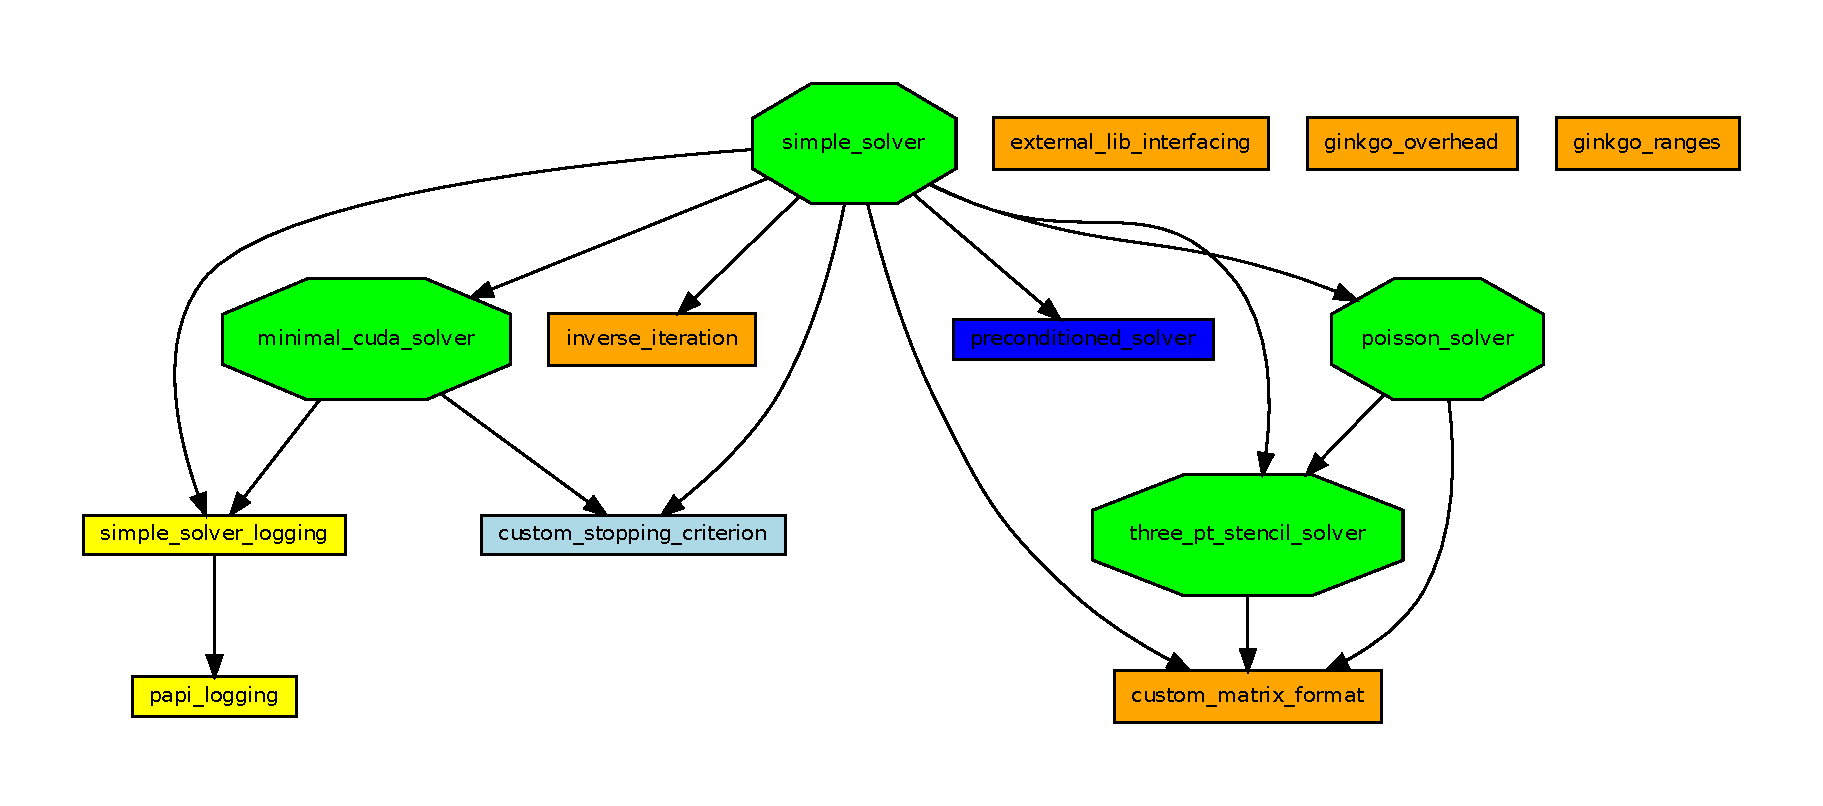
\includegraphics[width=\textwidth,height=\textheight/2,keepaspectratio=true]{dot_inline_dotgraph_1}}
\end{DoxyImageNoCaption}


{\bfseries Legend\+:}~\newline
 
\begin{DoxyImageNoCaption}
  \mbox{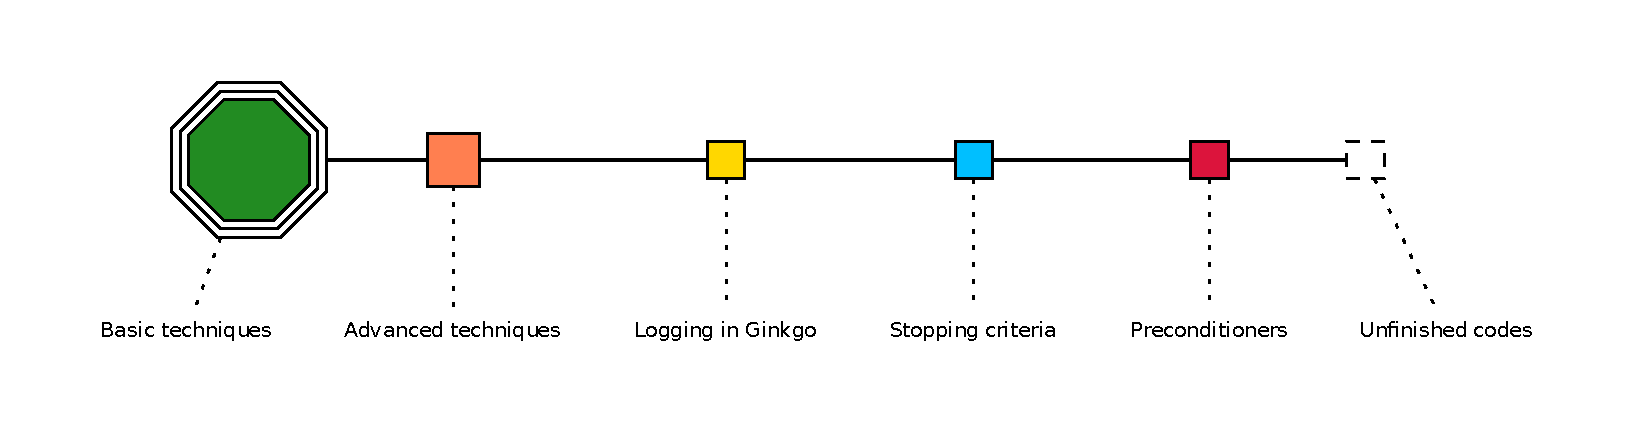
\includegraphics[width=\textwidth,height=\textheight/2,keepaspectratio=true]{dot_inline_dotgraph_2}}
\end{DoxyImageNoCaption}


\label{_list}%
 \subsubsection*{Example programs listed by number}

\tabulinesep=1mm
\begin{longtabu} spread 0pt [c]{*{2}{|X[-1]}|}
\hline
\hyperlink{simple_solver}{The simple-\/solver program} &Simple solver. A minimal CG solver in Ginkgo. Read matrix from a file. 

\\\cline{1-2}
\hyperlink{minimal_cuda_solver}{The minimal-\/cuda-\/solver program} &A first step solver with C\+U\+DA. Solve a linear system on N\+V\+I\+D\+IA G\+PU\textquotesingle{}s. 

\\\cline{1-2}
\hyperlink{poisson_solver}{The poisson-\/solver program} &Solve an actual physically relevant problem. Solving the poisson problem. Generate matrix within Ginkgo. 

\\\cline{1-2}
\hyperlink{preconditioned_solver}{The preconditioned-\/solver program} &Using a preconditioner for a linear system solve. Using the Jacobi preconditioner. 

\\\cline{1-2}
\hyperlink{three_pt_stencil_solver}{The three-\/pt-\/stencil-\/solver program} &Using a stencil to solve the poisson equation. Using array views. 

\\\cline{1-2}
\hyperlink{external_lib_interfacing}{The external-\/lib-\/interfacing program} &Interfacing with an external library. Using ginkgo\textquotesingle{}s solver with deal.\+ii. 

\\\cline{1-2}
\hyperlink{custom_matrix_format}{The custom-\/matrix-\/format program} &Creating a matrix-\/free stencil solver. Using ginkgo\textquotesingle{}s advanced methods to create your own custom matrix format to create a matrix free solver. 

\\\cline{1-2}
\hyperlink{inverse_iteration}{The inverse-\/iteration program} &Using Ginkgo to compute eigenvalues of a matrix with the inverse iteration method. 

\\\cline{1-2}
\hyperlink{simple_solver_logging}{The simple-\/solver-\/logging program} &Using the logging functionality in ginkgo to get solver and other information to diagnose and debug your code. 

\\\cline{1-2}
\hyperlink{papi_logging}{The papi-\/logging program} &Using the P\+A\+PI logging library in Ginkgo to get advanced information about your code and its behaviour. 

\\\cline{1-2}
\hyperlink{ginkgo_overhead}{The ginkgo-\/overhead program} &Measuring the overhead of the ginkgo library. 

\\\cline{1-2}
\hyperlink{custom_stopping_criterion}{The custom-\/stopping-\/criterion program} &Creating a custom stopping criterion for the iterative solution process. 

\\\cline{1-2}
\hyperlink{ginkgo_ranges}{The ginkgo-\/ranges program} &Using the ranges concept to factorize a matrix with the LU factorization. 

\\\cline{1-2}
\end{longtabu}


\label{_topic}%
 \subsubsection*{Example programs grouped by topics}

\paragraph*{{\bfseries Basic techniques}}

\tabulinesep=1mm
\begin{longtabu} spread 0pt [c]{*{2}{|X[-1]}|}
\hline
Solving a simple linear system with choice of executors.  &\hyperlink{simple_solver}{The simple-\/solver program}  

\\\cline{1-2}
Using the C\+U\+DA executor  &\hyperlink{minimal_cuda_solver}{The minimal-\/cuda-\/solver program}  

\\\cline{1-2}
Using preconditioners  &\hyperlink{preconditioned_solver}{The preconditioned-\/solver program}  

\\\cline{1-2}
Solving a physically relevant problem  &\hyperlink{poisson_solver}{The poisson-\/solver program}, \hyperlink{three_pt_stencil_solver}{The three-\/pt-\/stencil-\/solver program}, \hyperlink{custom_matrix_format}{The custom-\/matrix-\/format program}  

\\\cline{1-2}
Reading in a matrix and right hand side from a file.  &\hyperlink{simple_solver}{The simple-\/solver program}, \hyperlink{minimal_cuda_solver}{The minimal-\/cuda-\/solver program}, \hyperlink{preconditioned_solver}{The preconditioned-\/solver program}, \hyperlink{inverse_iteration}{The inverse-\/iteration program}, \hyperlink{simple_solver_logging}{The simple-\/solver-\/logging program}, \hyperlink{papi_logging}{The papi-\/logging program}, \hyperlink{custom_stopping_criterion}{The custom-\/stopping-\/criterion program}  

\\\cline{1-2}
\end{longtabu}


\paragraph*{{\bfseries Advanced techniques}}

\tabulinesep=1mm
\begin{longtabu} spread 0pt [c]{*{2}{|X[-1]}|}
\hline
Using ginkgo with external libraries.  &\hyperlink{external_lib_interfacing}{The external-\/lib-\/interfacing program}  

\\\cline{1-2}
Writing your own matrix format  &\hyperlink{custom_matrix_format}{The custom-\/matrix-\/format program}  

\\\cline{1-2}
Using Ginkgo to construct more complex linear algebra routines.  &\hyperlink{inverse_iteration}{The inverse-\/iteration program}  

\\\cline{1-2}
Logging within Ginkgo.  &\hyperlink{simple_solver_logging}{The simple-\/solver-\/logging program}, \hyperlink{papi_logging}{The papi-\/logging program}  

\\\cline{1-2}
Constructing your own stopping criterion.  &\hyperlink{custom_stopping_criterion}{The custom-\/stopping-\/criterion program}  

\\\cline{1-2}
Using ranges in Ginkgo.  &\hyperlink{ginkgo_ranges}{The ginkgo-\/ranges program}   \\\cline{1-2}
\end{longtabu}
